\chapter{Etude de cas - défaillance circuit intégré}
\label{chap:3}
\section{Présentation du produit et de la défaillance}

Description du produit

%TODO short intro

% What kind of product
An automotive \gls{asic} is tested to highlight a practical case of functional failure.
The studied chip performs several high-level and critical functions for the car vehicle.
The input used during the tests to inject the \gls{esd} inside the system is the battery supply connection (Fig. \ref{fig:system_architecture}).

\begin{figure}[!h]
  \centering
  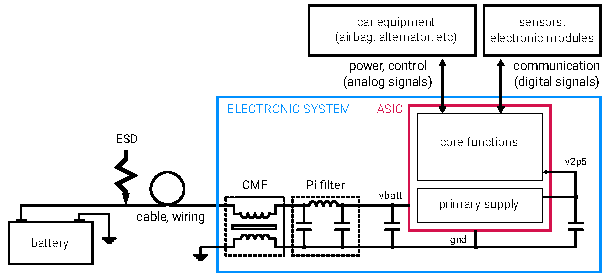
\includegraphics[width=0.9\textwidth]{src/3/figures/architecture_system.pdf}
  \caption{Overview of the system architecture}
  \label{fig:system_architecture}
\end{figure}

% Main task
The main function of the regulation function is to down-convert a battery voltage to a 2.5V regulated supply.
Several blocks are involved for processing the battery supply.
The overall architecture is given in fig. \ref{fig:monitored_function}).

\begin{figure}[!h]
  \centering
  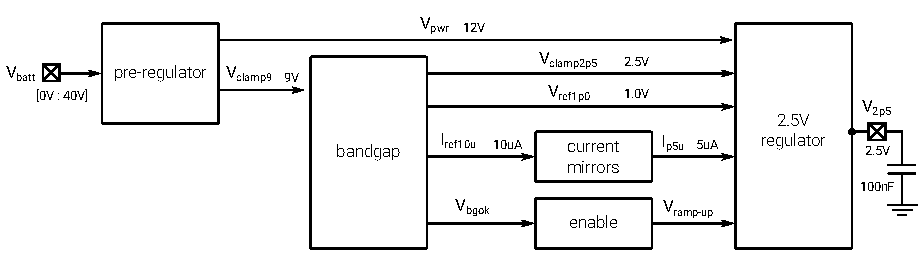
\includegraphics[width=0.9\textwidth]{src/3/figures/monitored_function.pdf}
  \caption{Architecture of the primary supply}
  \label{fig:monitored_function}
\end{figure}

%TODO simplifier
% First block
First, a pre-regulator clamps the battery input (V\textsubscript{batt}) that can reach up to 40V and down to 9V.
This is done to protect more sensitive circuitry connected downstream.
This clamped voltage is accessible on output V\textsubscript{clamp9}.
V\textsubscript{clamp9} has low current capability and is used for low-power functions.
A second output V\textsubscript{pwr} provides a 12V clamped output with a large current capability.
% Second block
A bandgap reference is connected downstream.
It is powered with V\textsubscript{clamp9}.
Once properly started after a certain delay, the bandgap generates a 1.0 V voltage reference on V\textsubscript{ref1p0}.
This reference is stable accross a wide range of temperature, process variation and process mismatchs.
The bandgap also outputs a 10uA current reference on I\textsubscript{ref10u}, and a flag V\textsubscript{bgok} to signal it is ready for operation.
% Third major block
Finally, the \gls{ldo} regulator generates a stable 2.5V supply voltage on V\textsubscript{2p5}.
This output can deliver up to 20mA.
V\textsubscript{2p5} is used further in the system to power digital gates.

Présentation de la défaillance

The failure is observed on the V\textsubscript{2p5} output pin (Fig. \ref{fig:meas-reset-v2p5}).
It affects the behavior of the entire system, because this net powers many other functions in the system.
The failure is induced by injecting a large negative-voltage stress on the input V\textsubscript{batt}, when the product is in operation.
The discharge is superimposed on a DC voltage value.
This input is a realistic entry point for \gls{esd} in the integrated circuit, because it is exposed at the system level and connected to the battery by a cable.
The disturbance on the output V\textsubscript{2p5} is much longer (30 \textmu{}s) than on the input V\textsubscript{batt} (100 ns).
It seems the negative stress is triggering a reset of the regulator.

\begin{figure}[!h]
  \centering
  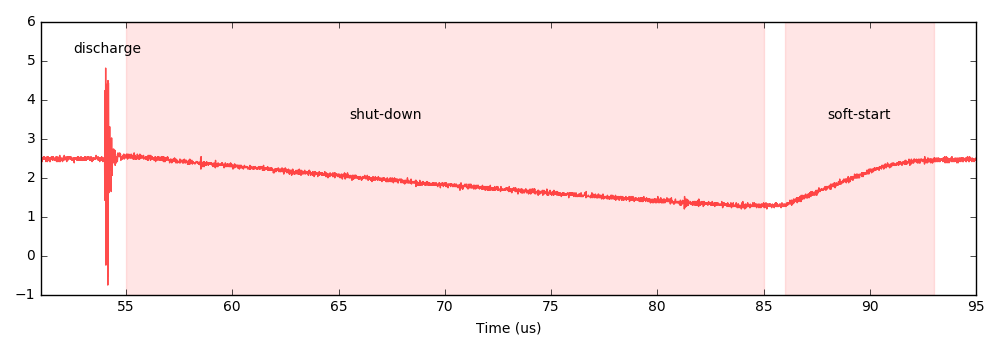
\includegraphics[width=0.9\textwidth]{src/3/figures/v2p5_measure.png}
  \caption{Measurement of V\textsubscript{2p5} after a -450V 100ns negative stress}
  \label{fig:meas-reset-v2p5}
\end{figure}

% What is the root cause -> reset of regulator, soft-start
It seems that the negative stress is causing an unwanted \gls{soft-start} sequence in the regulator.
A soft-start normally happens only during system power-up, when the main external supply is switched on.
During a soft-start, the supply voltage slowly rises from 0V to its nominal value.
It avoids overshoots that could damage sensitive blocks.
By design, soft-starts require a large amount of time to complete, in the range of tens to hundreds microseconds.
As a consequence, the function is not available, or at least not considered valid, until the soft-start is finished.

The next part of this research work is focused on developping measurement methods to acquire data on silicon, to confirm the simulations.
A testchip is designed to test new measurement and observation methods in section \ref{sec:test-vehicle-desc}.
Modeling methods are explored in section \ref{sec:bottom-up-modeling} as a way to understand and predict these functional issues.

\section{Présentation du véhicule de test}

Architecture et vue top du véhicule de test

% Global architecture
The global architecture of the testchip (Fig. \ref{architecture_testchip}) is comprised of a duplicated supply function.
The same supply block is instanciated twice on silicon.
One of them is the function under test, which is exposed to \gls{ESD} stresses and is monitored for failures.
The second one is responsible for powering the monitoring functions.

\begin{figure}[h]
  \centering
  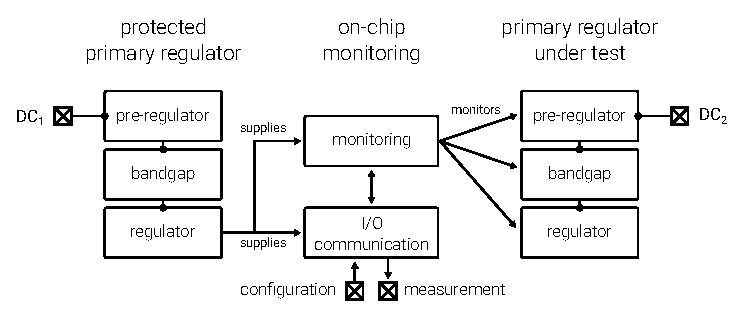
\includegraphics{src/3/figures/architecture_testchip.pdf}
  \caption{Global architecture of the test vehicle}
  \label{architecture_testchip}
\end{figure}

% What is in the monitoring system
The \textit{monitoring system} is comprised of several functions.
The overvoltage and undervoltage detectors monitor multiple net voltages inside the supply under test.
There are in total 35 detectors in the testchip.
The communication function performs a parallel to serial conversion, in order to read and write a large amount of bits using just a few pins.
Special structures for specific monitoring functions is also implemented.
Details about the monitoring functions are given in the next sub-sections.

% intro
Except for the two supply blocks, all the functionnalities described previously were designed, simulated and layouted.
All layouts were assembled together to form the topcell (Fig. \ref{fig:top-cell-layout}).
The complete pinout is given in appendix \ref{apx:testchip-pinout}.

\begin{figure}[!h]
  \centering
  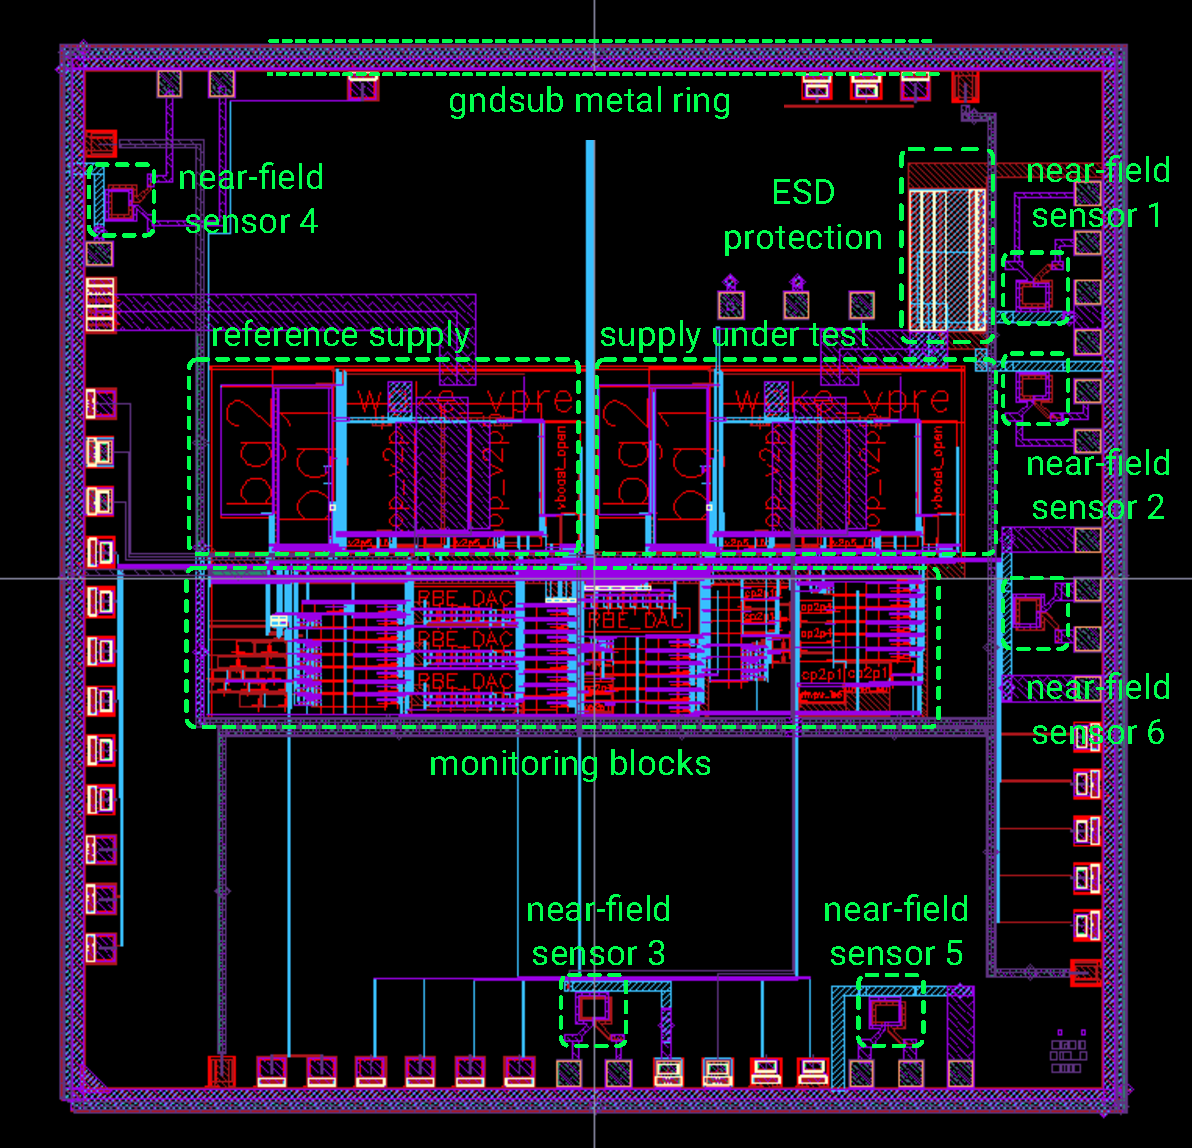
\includegraphics[width=0.7\textwidth]{src/3/figures/topcell_layout.pdf}
  \caption{Top-cell layout}
  \label{fig:top-cell-layout}
\end{figure}

% Talk about the near-field current sensors placement
In total, there are 6 near-field current sensors located on the device.
The 6\textsuperscript{th} sensor is dedicated to calibration.
The others are placed strategically on main \gls{io} susceptible to be disturbed directly or indirectly by \gls{esd}s.
Sensor \textit{1} measures the current on the supply under test power input.
During testing, this pin is be exposed to \gls{esd}s coupled on top of a DC supply voltage.
Internally, this input is protected by a large \gls{esd-protection}, able to sustain IEC 61000-4-2 \gls{esd-gun} discharges.
Sensor \textit{2} measures the current absorbed and deviated by the \gls{esd-protection} into the \textit{gndsub} metal ring (local ground reference).
Sensors \textit{3} measures the current flowing to the external stabilisation capacitor of the regulator under test.
Finally, sensors \textit{4} and \textit{5} measure the currents flowing from the \textit{gndsub} metal ring into the external ground pins, connected externally to the board ground.

% Explain why so much empty space
On the layout, a lot of silicon space was left empty.
This is due to manufacturing constraints that enforced the silicon dimensions.
After manufacturing and packaging, the chip is tested.
The entire testing process and results are documented in section \ref{sec:test-vehicle-testing}.

Description rapide des blocks désignés

% What are the OV/UV detectors made of
Overvoltage and undervoltage detectors are implemented as latched comparators.
A flag is raised if a monitored net crosses a threshold, and stored using a latch, until it can be read.
The architecture of a single detector is given Fig. \ref{fig:architecture-ov}.
The same architecture is used for the overvoltage and the undervoltage.
Monitored and reference inputs are just inversed on the undervoltage detector.

\begin{figure}[!h]
  \centering
  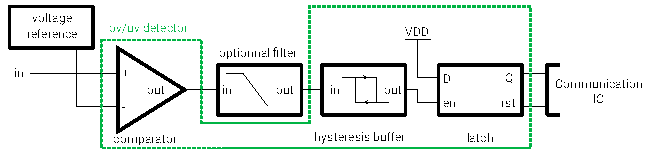
\includegraphics[width=0.9\textwidth]{src/3/figures/architecture_OV.pdf}
  \caption{Architecture of the overvoltage detector}
  \label{fig:architecture-ov}
\end{figure}

% Detail architecture
The first block in this detector is the comparator.
It is designed with a two-stage operational amplifier with an output buffer (see Fig. \ref{fig:comparator-design}).
This topology is well suited for high-gain, open-loop comparators.
This comparator provides a very high input impedance, to ensure the monitored net is not disturbed.
A high-gain is useful for limiting the comparator's offset.


% What is the purpose of filter
On the output of the comparator, an optional RC filter can be connected.
This filter can deglitch very short overvoltages, to only let large overvoltages pass through the detector.
The stratety behind this filter is to use multiple detectors monitoring the same net, each one with a different filter.
In function of which detectors triggered, an estimation of the overvoltage length can be made.

% Hysteresis buffer
After the filter, an hysteresis buffer increases the deglitching action of the filter.
If the comparator's output remains high for a short period of time, the output of the filter will rise slowly.
If a standard buffer was used in place of the hysteresis buffer, it would latch at about half the supply voltage.
With the hysteresis, the buffer switches at a voltage much closer from the supply.
With the same RC filter, this results in a much longer deglitching time.
This was done because RC-filters require large resistors and large capacitors for integration on silicon, and occupy a considerable area on the chip.
By increasing the deglitching time, smaller RC-filters could be used.

% Latch
Finally, the latch stores the overvoltage flag.
By default, the latch is reset at $t=0$.
Its copy input $D$ is connected to the supply.
If the hysteresis buffer triggers high, the enable pin triggers a copy in the latch.
The output $Q$ copies the value from the $D$, storing a logical high in the latch.

% Origin of reference voltages
The reference voltages for these comparators come from either fixed-values set by the protected supply, or \gls{dac} that can be reconfigured through the communication system.

%TODO introduce near field sensor

% What is a current sensors
In this testchip, the current sensor is a near-field current loop.
The sensor is placed close to a metal track in which current must be measured.
By coupling, the sensor generates a voltage proportional to the derivative of the current in the track.

Figure. \ref{fig:near-field-current-sensor} and \ref{fig:near-field-current-sensor-layout} gives respectively a visual representation of the sensor and the final layout.
This kind of integrated loop was originally designed and studied in \cite{AlainSallesInductors}.

\begin{figure}[!h]
  \centering
  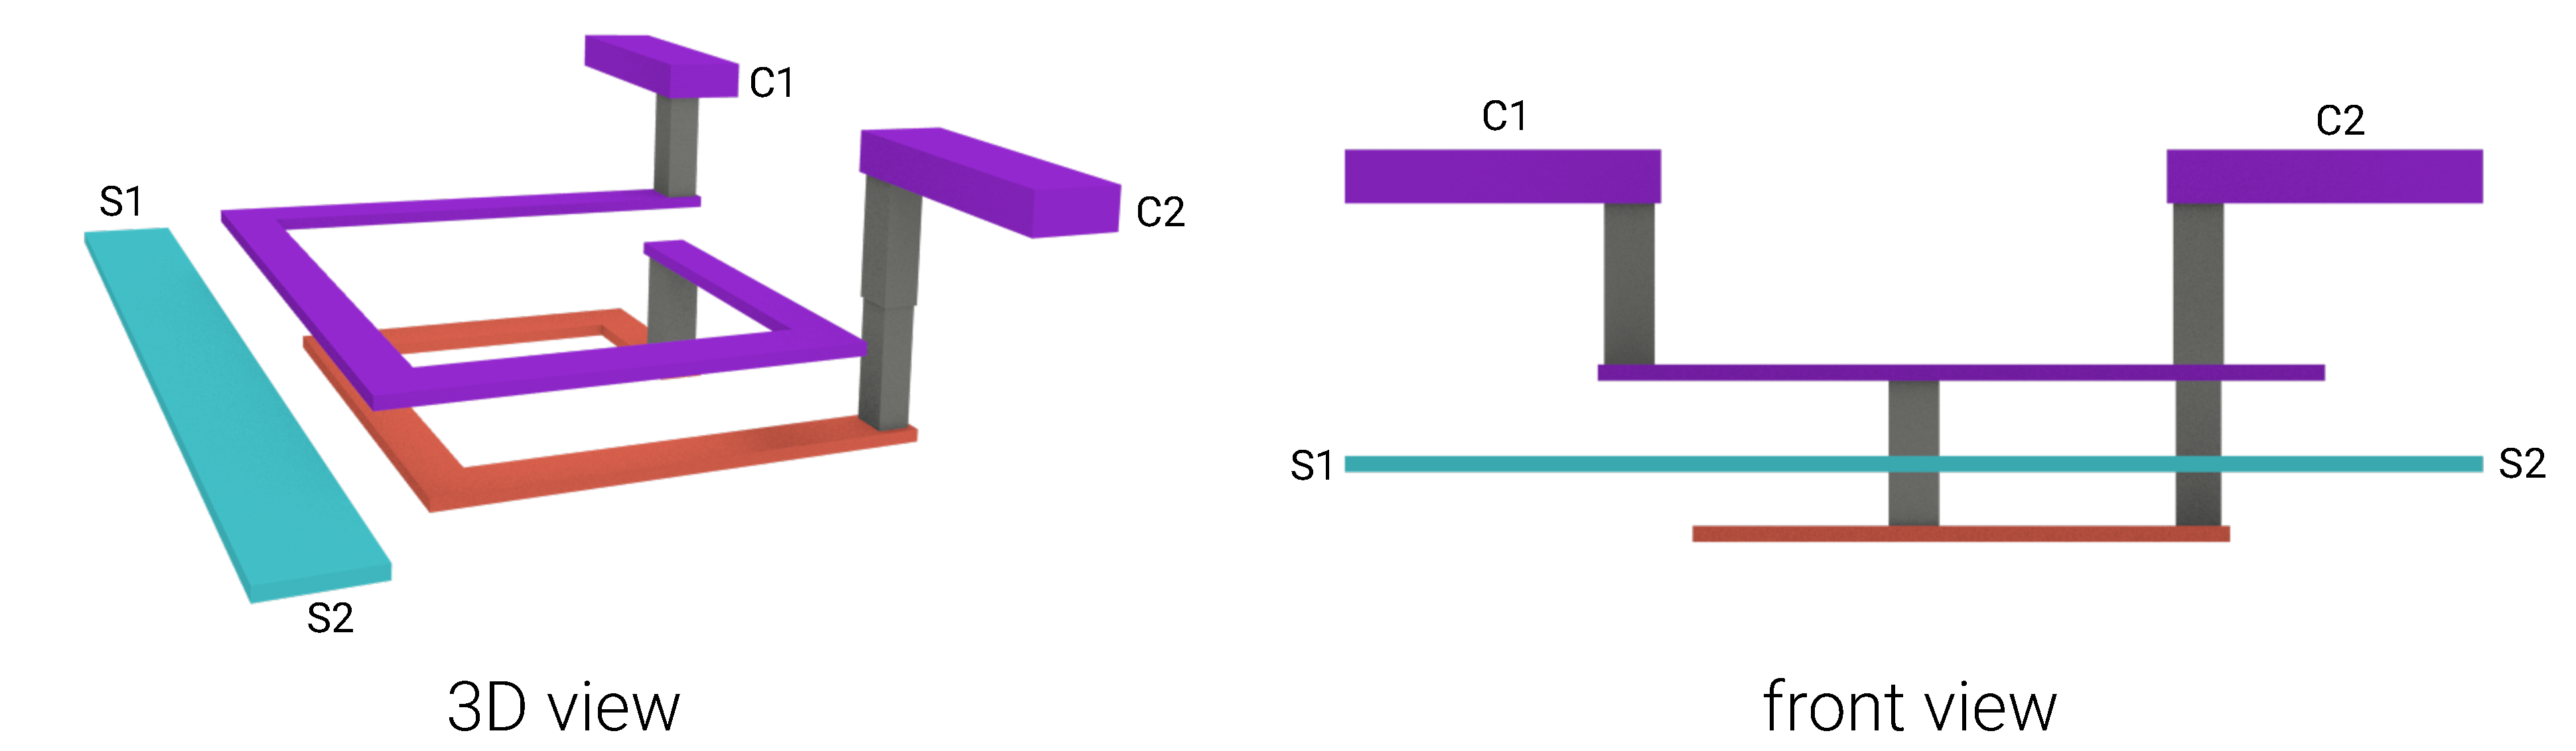
\includegraphics[width=0.98\textwidth]{src/3/figures/near-field-current-sensor.pdf}
  \caption{Near-field current sensor design}
  \label{fig:near-field-current-sensor}
\end{figure}

\begin{figure}[!h]
  \centering
  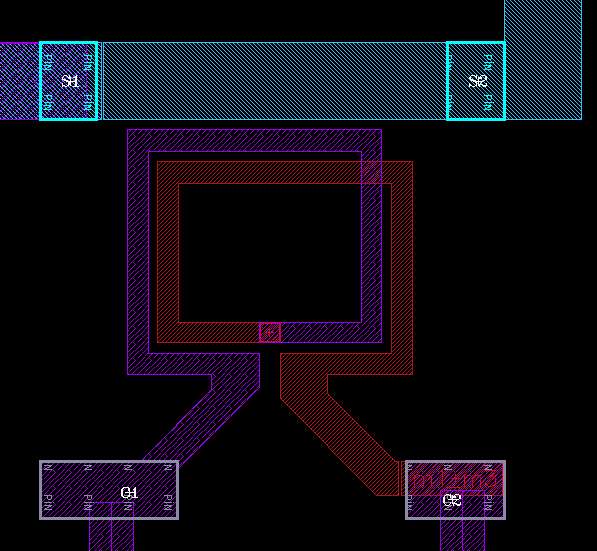
\includegraphics[width=0.5\textwidth]{src/3/figures/sensor_layout.png}
  \caption{Near-field current sensor layout}
  \label{fig:near-field-current-sensor-layout}
\end{figure}

% How is it designed and how is it used
On silicon, three levels of metal are used to build the sensor.
The first level (in red) and the third level (in purple) form a metal loop.
Metallic vias connect both levels to close the loop vertically.
Finally, the sensed current is at the second level (pale blue), and circulates between nets \textit{S1} and \textit{S2}.
An oscilloscope with 50\textOmega\ input impedance performs a differential voltage measurement between pins \textit{C1} and \textit{C2}.
An example waveform obtained by injecting a rectangular pulse is given in Fig. \ref{fig:nfs-wvf}.
The obtained waveform requires specific post-processing to reconstitute the original current waveform.
The post-processing is detailed later in section \ref{sec:on-chip-near-field-process}.
